\documentclass[12pt]{article}

\usepackage{breqn}
\usepackage[margin=1in]{geometry} 
\usepackage{amsmath,amsthm,amssymb,enumitem}
\usepackage[german,spanish,english]{babel}
\usepackage{tensor}
\usepackage{graphicx}
\usepackage{esint}
\usepackage[T1]{fontenc}
\usepackage{mathtools}
\usepackage{siunitx}
\newenvironment{ex}[2][Exercise]{\begin{trivlist}
\item[\hskip \labelsep {\bfseries #1}\hskip \labelsep {\bfseries #2.}]}{\end{trivlist}}

\newenvironment{sol}[1][Solution]{\begin{trivlist}
\item[\hskip \labelsep {\bfseries #1:}]}{\end{trivlist}}

\newcommand{\meq}{\overset{!}{=}}
\DeclarePairedDelimiter\bra{\langle}{\rvert}
\DeclarePairedDelimiter\ket{\lvert}{\rangle}
\DeclarePairedDelimiterX\brk[2]{\langle}{\rangle}{#1\,\delimsize\vert\,\mathopen{}#2}
\DeclareSIUnit\angstrom{\text {Å}}

%DECLARATION OF DELIMITERS%

\DeclarePairedDelimiter\vb{\lvert}{\rvert}
\DeclarePairedDelimiter\rb{(}{)}
\DeclarePairedDelimiter\sqrb{[}{]}
\DeclarePairedDelimiter\cb{\{}{\}}
\DeclarePairedDelimiter\ab{\langle}{\rangle}
\DeclarePairedDelimiter\db{\|}{\|}


\begin{document}
\noindent Richard Abele \hfill \today \\[30pt]
\centerline{ \Large{ \textbf{ Problem Set 8 - Ordinary Differntial Equations }}}

\begin{ex}
    1 Runge Kutta Proofs
\end{ex}

For this exercise we are asked to solve choose two of six possible exercises. The two exercises that I chose are as follows:

\begin{enumerate}[label=(\alph*)]
    \item Derive the 3rd order Runge-Kutta formula 
        \begin{align*}
            y_{n+1} & =  y_{n} + \frac{1}{9} \rb*{ 2 k_{1} + 3 k_{2} + 4 k_{3}}
        \end{align*}
        with
        \begin{align*}
            k_{1} & =  h f\rb*{x,y} &\\
            k_{2} & =  h f \rb*{x + \frac{1}{2} h, y + \frac{1}{2} k_{1}} &\\
            k_{3} & =  h f \rb*{ x + \frac{3}{4} h , y + \frac{3}{4} k_{2}}
        \end{align*}
    \item Prove that in the special case that \(y' = f\rb*{x}\) the 4th order RK formula is equivalent to Simpson's rule.
\end{enumerate}

\begin{sol} 1 \end{sol}

\begin{enumerate}[label=(\alph*)]
    \item The general form of a 3rd order RK method is given by the form
        \begin{align*}
            y_{n+1} & =  y_{n} + w_{1} k_{1} + w_{2} k_{2} + w_{3} k_{3}
        \end{align*}
        with \(w_{n}\) being weights and \(k_{n}\) being intermediate slopes. These \(k_{n}\) values are defined by the general form
        \begin{align*}
            k_{1} & =  h f \rb*{x_{n}, y_{n}} &\\
            k_{2} & =  h f \rb*{ x_{n} + \alpha_{2} h , y_{n} + \beta_{21} k_{1}} &\\
            k_{3} & =  h f \rb*{ x_{n} + \alpha_{3} h , y_{n} + \beta_{31} k_{1} + \beta_{32} k_{2}} &\\
        \end{align*}
        The values of \(w, k, \alpha, \text{and }, \beta\) are chosen to most closely approximate a Taylor of \(y_{n+1}\). The general Taylor expansion takes the following form:
        \begin{align*}
            y_{n+1} & =  y\rb*{x_{n+1}} = y \rb*{x_{n}} + h y'\rb*{x_{n}} 
            + \frac{h^{2}}{2} y''\rb*{x_{n}} + \frac{h^{3}}{6} y''' \rb*{x_{n}} + \mathcal{O} \rb*{h^{4}} &\\
        \end{align*}
        knowing that \(y' = \frac{d y}{d x} = f\), we can rewrite the derivatives of \(y\) as 
        \begin{align*}
            y'' \rb*{x} & =  \frac{d }{d x} f\rb*{x,y} = f_{x} + f_{y}y' = f_{x} + f_{y} f &\\
            y''' \rb*{x} & =  \frac{d }{d x} \rb*{f_{x} + f_{y} f} &\\
            & = f_{xx} + 2 f_{xy} f + f_{yy} f^{2} + f_{y} \rb*{f_{x} + f_{y} f} &\\
        \end{align*}
        with help from the chain rule in multivariable calculus. 

        We now continue by calculating the taylor series of the RK formula so that we can compare coefficients. We know that the general form for a Taylor series in two variables is 
        \begin{align*}
            f \rb*{x + h, y + k} & =  \sum_{i = 0}^{\infty} {\frac{1}{i!} \rb*{ h \frac{\partial }{\partial x} + k \frac{\partial }{\partial y}}^{i} f \rb*{x,y}}.  &\\
        \end{align*}
        Applying this formula we get
        \begin{align*}
            k_{2} & =  h [ f \rb*{x_{n}, y_{n}} + \alpha_{2} h f_{x} + \beta_{21} k_{1} f_{y} + \frac{1}{2} \rb*{ \alpha_{2} h}^{2} f_{xx}
            + \alpha_{2} h \beta_{21} k_{1} f_{xy} &\\
            & \hspace{20pt}+ \frac{1}{2} \rb*{\beta_{21} k_{1}}^{2} f_{yy} + \dots  ] &\\
            k_{3} & =  h [ f \rb*{x_{n}, y_{n}} + \alpha_{3} h f_{x} + \rb*{\beta_{31} k_{1} + \beta_{32} k_{2}} f_{y} 
            + \frac{1}{2} \rb*{\alpha_{3} h }^{2} f_{xx} &\\
             & \hspace{20px}+ \alpha_{3} h \rb*{ \beta_{31} k_{1} + \beta_{32} k_{2}} f_{xy}
            + \frac{1}{2} \rb*{ \beta_{31}k_{1} + \beta_{32} k_{2}}^{2} f_{yy} + \dots  ]&\\
        \end{align*}
        Comparing the values of \(h, h^{2}, h^{3}, \text{and } h^{4}\), we can develop the following system of equations: 
        \begin{align*}
            w_{1} + w_{2} + w_{3} & =  1 &\\
            w_{2} \alpha_{2} + w_{3} \alpha_{3} = \frac{1}{2} &\\
            w_{2} \alpha_{2}^{2} + w_{3} a_{3}^{2} = \frac{1}{3} &\\
            w_{3} \beta_{32} \alpha_{2} = \frac{1}{6} &\\
        \end{align*}
        From the specific formulations of \(k_{i}\) in the assignment we see that 
        \begin{align*}
            \alpha_{2} & =  \frac{1}{2}, \alpha_{3}  = \frac{3}{4}
            , \beta_{21} = \frac{1}{2}, \beta_{31} = 0, 
            \beta_{32} = \frac{3}{4}. &\\
        \end{align*}
        Inserting these values into the above system of equations leads to
        \begin{align*}
            w_{1} + w_{2} + w_{3} & = 1 &\\
            \frac{1}{2} w_{2} + \frac{3}{4} w_{3} & =  \frac{1}{2} &\\
            \rb*{\frac{1}{2}}^{2} w_{2} + \rb*{\frac{3}{4}}^{2} w_{3} & =  \frac{1}{3} &\\
            \frac{3}{4} \cdot \frac{1}{2} w_{3} & =  \frac{1}{6}. &\\
        \end{align*}
        Solving this system of equations yields
        \begin{align*}
            w_{1} & =  \frac{2}{9} &\\
            w_{2} & =  \frac{1}{3} &\\
            w_{3} & =  \frac{4}{9}. &\\
        \end{align*}
        When these values are instulted into the RK formula, we finally obtain
        \begin{align*}
            y_{n+1} & =  y_{n} + \frac{2}{9} k_{1} + \frac{1}{3} k_{2} + \frac{4}{9} k_{3} &\\
            & =  y_{n} + \frac{1}{9} \rb*{ 2 k_{1} + 3 k_{2} + 4 k_{3}} &\\
        \end{align*}
        as desired.
    \item 
        Given that \(y' = f \rb*{x}\), we can say that 
        \begin{align*}
            y_{n+1 } & =  y_{n} + \int_{x_{n}}^{x_{n+1}} { f \rb*{x}} \,d x &\\
        \end{align*}
        We want to show that the above integral approximation using RK4 is equal to the approximation given by Simpson's Rule:
        \begin{align*}
            \int_{x_{n}}^{x_{n+1}} f \rb*{x} dx & \approx
            {\frac{h}{6}
            \rb*{ f \rb*{x_{n}} + 4 f \rb*{x_{n} + \frac{h}{2}} + 
        f \rb*{ x_{n+1}}}} &\\
        \end{align*}
        We begin by writing the RK4 method for \(y' = f \rb*{x}\):
        \begin{align*}
            y_{n+1} & =  y_{n} + \frac{1}{6} \rb*{
                k_{1} + 2 k_{2} + 2 k_{3} + k_{4}
            }
        \end{align*}
        with
        \begin{align*}
            k_{1} & =  h f \rb*{x_{n}} &\\
            k_{2} & =  h f \rb*{x_{n} + \frac{h}{2}} &\\
            k_{3} & =  h f \rb*{x_{n} + \frac{h}{2}} &\\
            k_{4} & =  h f \rb*{ x_{n} + h} &\\
        \end{align*}
        Substituting in the values of \(k\) and combining like-terms, we obtain
        \begin{align*}
            y_{n+1} & =  y_{n} + \frac{h}{6} \rb*{ f \rb*{x_{n}}
            + 4 f \rb*{x_{n} + \frac{h}{2}} + f \rb*{x_{n} + h}} &\\
        \end{align*}
        Comparing the above expression to Simpson's Rule, we immediately see that they are equivalent, thus completing the proof.
\end{enumerate}

\newpage

\begin{ex}
    2 1st Order ODEs
\end{ex}

Consider the Initial Value Problems (INPs) for the 1st order differential equations below. Solve them for the interval \(x \in \sqrb*{0,30}\) using the Heun's, RK4, and Adams methods. 

\begin{enumerate}[label=(\alph*)]
    \item \(y' = y \cos \rb*{x + y}, y \rb*{0} = 1 \)
    \item \(y' = \sin \rb*{xy} \cos x + y  , y \rb*{0} = 1\)
    \item \(y' = xy - x^{2}, y \rb*{0} = 1\)
    \item \(y' = y \rb*{3 - y}, y \rb*{0} = 1\)
    \item \(y' = y^{2} - x^{2}, y\rb*{0} = \frac{1}{2}\)
    \item \(y' = \frac{1}{3x - 2y + 1}, y\rb*{0} = 0\)
\end{enumerate}


\begin{sol} 2 \end{sol}

The RK4, Heun, and Adams methods were implemented in C code and plotted with a Gnuplot script, both of which can be found in the \texttt{problem2} directory. The implemented routines are summarized below with a stepsize \(h\).

The general form of RK4 is given by the following formula:
\begin{align*}
    y_{n+1} & =  y_{n} + \frac{1}{6} \rb*{
    k_{1} + 2 k_{2} + 2 k_{3} + k_{4}} + \mathcal{O} \rb*{h^{5}} &\\
\end{align*}
with 
\begin{align*}
    k_{1} & =  h f \rb*{x_{n}, y_{n}} &\\
    k_{2} & =  h f \rb*{x_{n} + \frac{1}{2} h, y_{n} + \frac{1}{2} k_{1}}&\\
    k_{3} & =  h f \rb*{x_{n} + \frac{1}{2} h, y_{n} + \frac{1}{2} k_{2}} &\\
    k_{4} & = h f \rb*{x_{n} + h, y_{n} + k_{3}} &\\
\end{align*}

Heun's method can implemented by first finding an intermediate \(\tilde{y}_{i+1}\) and then calculating the final approximation \(y_{i+1}\) as follows:
\begin{align*}
    \tilde{y}_{i+1} & =  y_{i} + h f \rb*{t_{i}, y_{i}} &\\
    y_{i+1} & =  y_{i} + \frac{h}{2} \sqrb*{ f \rb*{t_{i}, y_{i}} + f \rb*{ t_{i+1} , \tilde{y}_{i+1}}} &\\
\end{align*}

Finally, Adams' method is given by the scheme
\begin{align*}
    y_{n+1} & =  y_{n} + \frac{h}{2} \rb*{y'_{n} + y'_{n+1} } &\\
\end{align*}

The equations were numerically solved using \(n = 1000\) steps and plotted below.

\begin{figure}[ht]
    \centering
    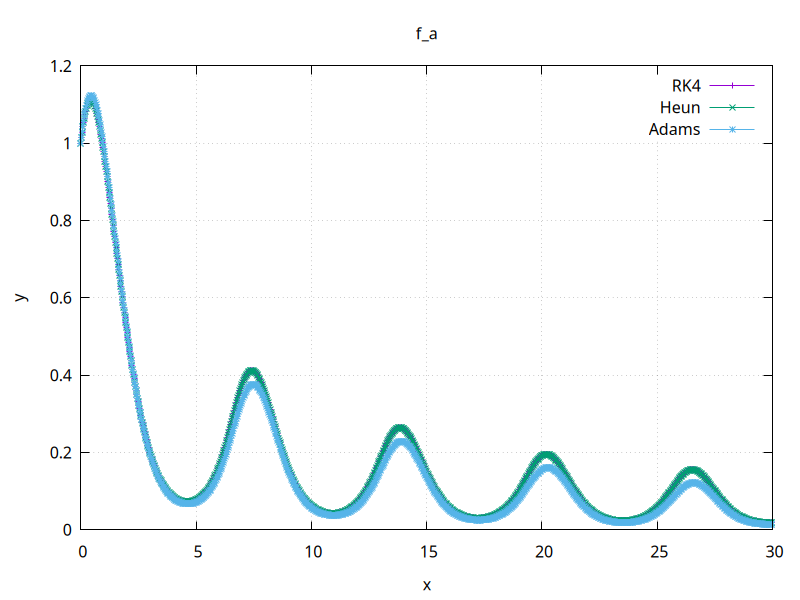
\includegraphics[width=0.75\textwidth]{./../problem2/data/f_a.png}
    \caption{Function A}
    \label{fig:fncA}
\end{figure}

\begin{figure}[ht]
    \centering
    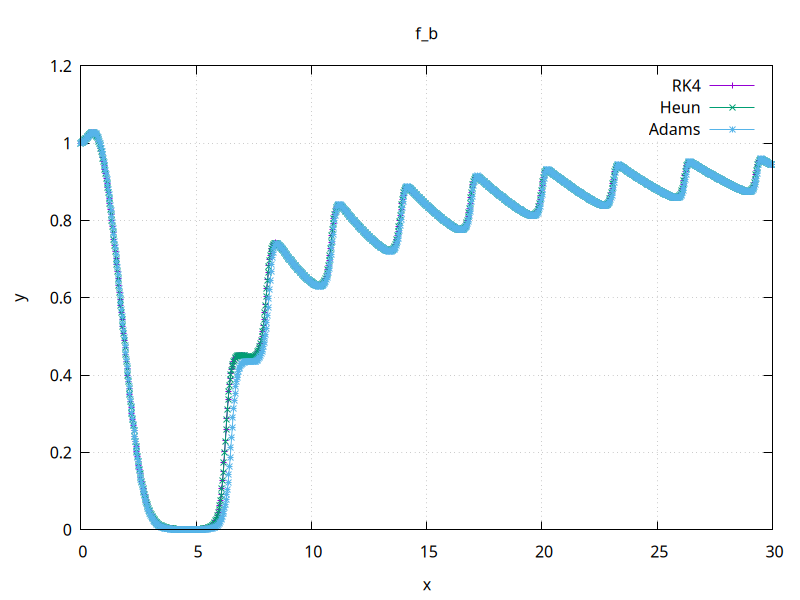
\includegraphics[width=0.75\textwidth]{./../problem2/data/f_b.png}
    \caption{Function B}
    \label{fig:fncB}
\end{figure}

\begin{figure}[ht]
    \centering
    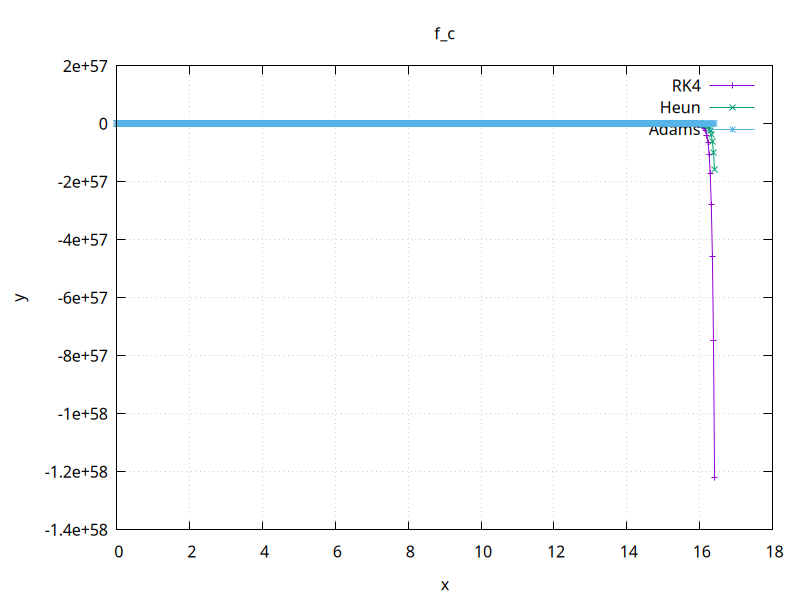
\includegraphics[width=0.75\textwidth]{./../problem2/data/f_c.png}
    \caption{Function C}
    \label{fig:fncC}
\end{figure}

\begin{figure}[ht]
    \centering
    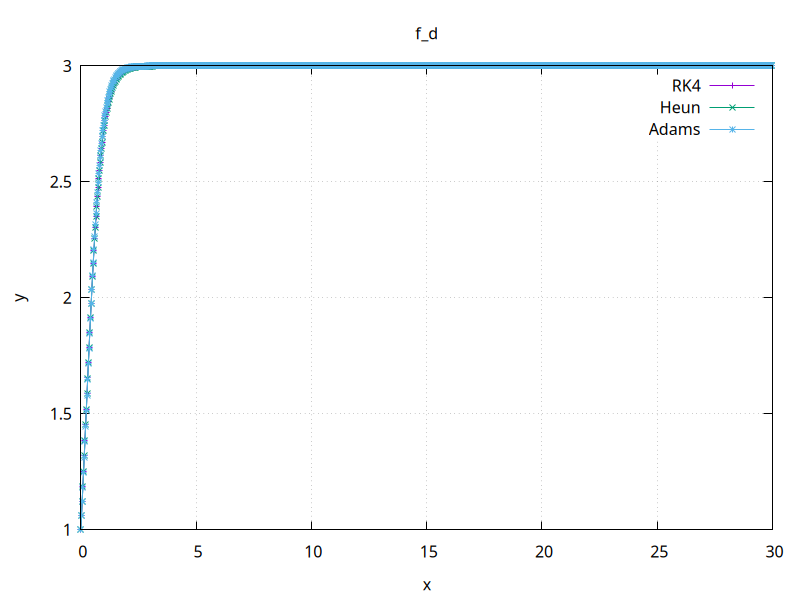
\includegraphics[width=0.75\textwidth]{./../problem2/data/f_d.png}
    \caption{Function D}
    \label{fig:fncD}
\end{figure}

\begin{figure}[ht]
    \centering
    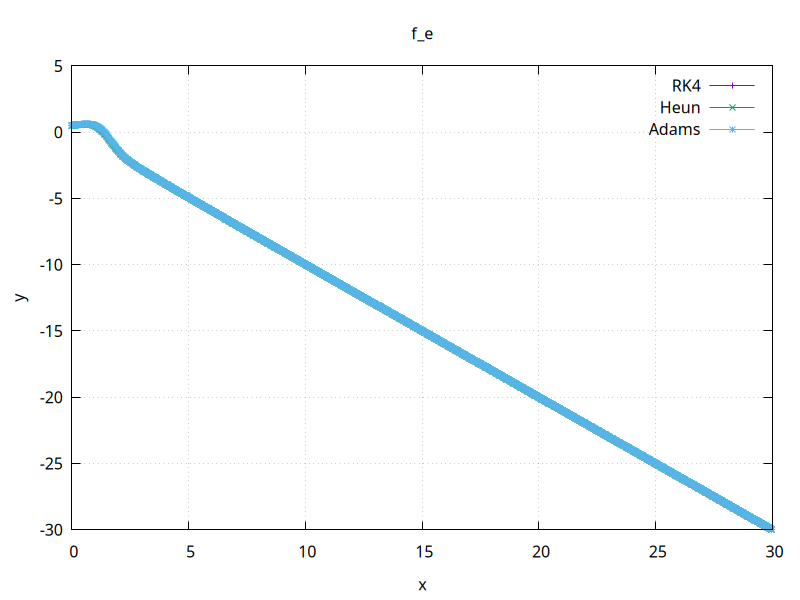
\includegraphics[width=0.75\textwidth]{./../problem2/data/f_e.png}
    \caption{Function E}
    \label{fig:fncE}
\end{figure}

\begin{figure}[ht]
    \centering
    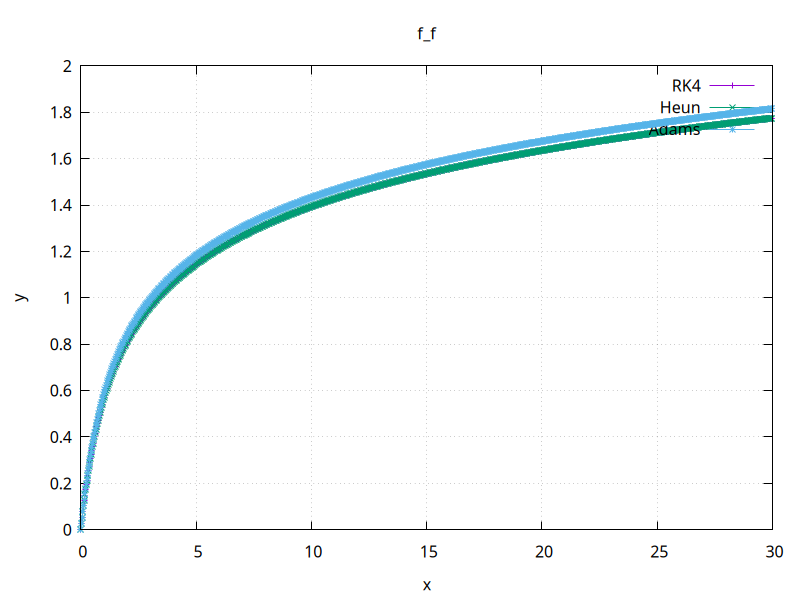
\includegraphics[width=0.75\textwidth]{./../problem2/data/f_f.png}
    \caption{Function F}
    \label{fig:fncF}
\end{figure}

\newpage

\begin{ex}
    3 - Nonlinear ODEs
\end{ex}

For this problem we consider Bernoulli non-linear ODEs in the form
\begin{align*}
    y'\rb*{x} & =  b \rb*{x} y^{\alpha}\rb*{x} + a \rb*{x} y \rb*{x} &\\
\end{align*}
with a constant \(\alpha > 0\).

Write a program to numerically integrate a single first-order ODE using 
\begin{itemize}
    \item RK4
    \item Adams-Moulton, without a corrective step
    \item Adams-Moulton with a corrective step
\end{itemize}

\begin{enumerate}[label=(\alph*)]
    \item 
Test the program on the DE 
\begin{align*}
    y' & =  y + x^{2} - 2 x + \sin \rb*{x} &\\ 
\end{align*}
with \(y_{0} = 0.1\) on the interval \(x \in \sqrb*{0,2}\).
     \begin{enumerate}[label=(\roman*)]
        \item Plot the absolute analytical error, \(E\) at \(x = 2\) as a function of the number of steps taken \(N \in \sqrb*{10, 5000}\) in a log-plot and discuss the convergence order.
        \item Plot the error vs the number of function evaluations (\(4N\) for RK4, \(N\) for Adams without corrections, \(2 N\) as a minimum for Adams with corrections). Which method is the most efficient? 
     \end{enumerate}
\item The evolution of the velocity of a body flowing through a non-ideal fluid can be described by a Bernouilli DE
    \begin{align*}
        v' \rb*{t} + \mu \rb*{t} v \rb*{t} - \omega \rb*{ t}^{2} v^{3} \rb*{t} & =  0 &\\
    \end{align*}
    with \(\omega\rb*{t}\) and \(\mu\rb*{t}\) being two positive functions. Assume the initial condition \(v_{0} = 2\).
    \begin{enumerate}[label=(\roman*)]
        \item Plot the absolute analytical error at \(t = 1.5\) with the constant parameters \(\omega \rb*{ t } = \omega_{0} = 0.707\), \(\mu \rb*{t} = \mu_{0} = 2\).
        \item Keep \(\mu_{0} = 2\) constant and vary \(\omega_{0}\) in the vicinity of \(\frac{1}{\sqrt{2}}\). How does the solution behave? 
        \item Consider \(\omega \rb*{t} = \omega_{0} \tan \rb*{t} \) with \(\omega_{0} = \frac{1}{\sqrt{2}}\) and \(\mu_{0} = 2\) initially. Slowly increase \(\mu_{0}\) towards 1.5 - comment on what you see.
    \end{enumerate}
\end{enumerate}

\begin{sol} 3 \end{sol}
To solve this problem the code from \texttt{problem2} was copied and expanded. The methology of RK4 is explained in the previous problems on this sheet. The Adams-Moulton method for ODEs is given by
\begin{align*}
    y_{k+1} & =  y_{k} + \frac{h}{24} \rb*{ 9 f_{k+1} + 19 f_{k} - 5 k_{k - 1} + f_{k-2}} + \mathcal{O} \rb*{h^{5}} &\\
\end{align*}
\(f_{k+1}\) of course depends on \(y_{k+1}\), making this an implicit method. This can be remedied by using predictor-corrector techniques, such as evaluating \(y_{k+1}\) as 
\begin{align*}
    y_{k+1} & =  y_{k} + \frac{h}{24} \rb*{ 55 f_{k}  - 59 f_{k - 1} + 37 f_{k - 2} - 9 f_{k - 3}} + \mathcal{O} \rb*{h^{5}}. &\\
\end{align*}




\end{document}
